\chapter{Event selection in ND-GAr}
\label{chapter:gar_selection}

\section{Data sample}

\begin{table}[t]
	\caption{Event rates in ND-GAr.}
	\begin{center}
		\begin{small}
			\begin{tabular}{lcc}
                & \multicolumn{2}{c}{Events/ton/year}                                                                   \\[2mm] \cline{2-3} 
            \multicolumn{1}{c}{\rule{0pt}{1.1\normalbaselineskip}Process}       & $1.1 \times 10^{21} ~ \mathrm{POT}/\mathrm{year}$ & $1.9 \times 10^{21} ~ \mathrm{POT}/\mathrm{year}$ \\[2mm] \hline
            \rule{0pt}{1.1\normalbaselineskip}All $\nu_{\mu}$-CC                & $1.60 \times 10^{6}$                              & $2.83 \times 10^{6}$                              \\[2mm]
            $\hspace{0.5 cm}$ CC $0\pi$       & $5.28 \times 10^{5}$                              & $9.35 \times 10^{5}$                              \\[2mm]
            $\hspace{0.5 cm}$ CC $1\pi^{\pm}$ & $3.02 \times 10^{5}$                              & $5.34 \times 10^{5}$                              \\[2mm]
            $\hspace{0.5 cm}$ CC $1\pi^{0}$   & $1.65 \times 10^{5}$                              & $2.92 \times 10^{5}$                              \\[2mm]
            $\hspace{0.5 cm}$ CC $2\pi$       & $3.18 \times 10^{5}$                              & $5.63 \times 10^{5}$                              \\[2mm]
            $\hspace{0.5 cm}$ CC $3\pi$       & $1.36 \times 10^{5}$                              & $2.41 \times 10^{5}$                              \\[2mm]
            $\hspace{0.5 cm}$ CC other        & $1.52 \times 10^{5}$                              & $2.69 \times 10^{5}$                              \\[2mm] \hline
            \rule{0pt}{1.1\normalbaselineskip}All $\bar{\nu}_{\mu}$-CC          & $7.54 \times 10^{4}$                              & $1.33 \times 10^{5}$                              \\[2mm]
            All NC                            & $5.50 \times 10^{5}$                              & $9.73 \times 10^{5}$                              \\[2mm]
            All $\nu_{e}$-CC                  & $2.70 \times 10^{4}$                              & $4.78 \times 10^{4}$                             
            \end{tabular}
		\end{small}
	\end{center}
	\label{tab:ndgar_event_rates}
\end{table}

\section[\texorpdfstring{$\nu_{\mu}$}{numu} CC selection]{\boldmath\texorpdfstring{$\nu_{\mu}$}{numu} CC selection}

In some cases, it is interesting to divide the signal events by interaction mode. I will distinguish between charged-current quasi-elastic (CCQE), coherent (CCCOH), resonant (CCRES), and deep-inelastic (CCDIS) interactions. I also use a separate category for the interactions not included in any of the others (CCOther).

For this selection, I use the following categorisation for the background events:
\begin{itemize}
    \item Out of FV: if the true neutrino vertex lies outside the defined FV.
    \item NC: if the event is a true neutral-current event.
    \item $\bar{\nu}_{\mu}$ CC: if the true neutrino candidate is of muon antineutrino flavour.
    \item Other: if the event is not signal nor falls in any of the other background categories.
\end{itemize}

\begin{figure}[t]
\centering
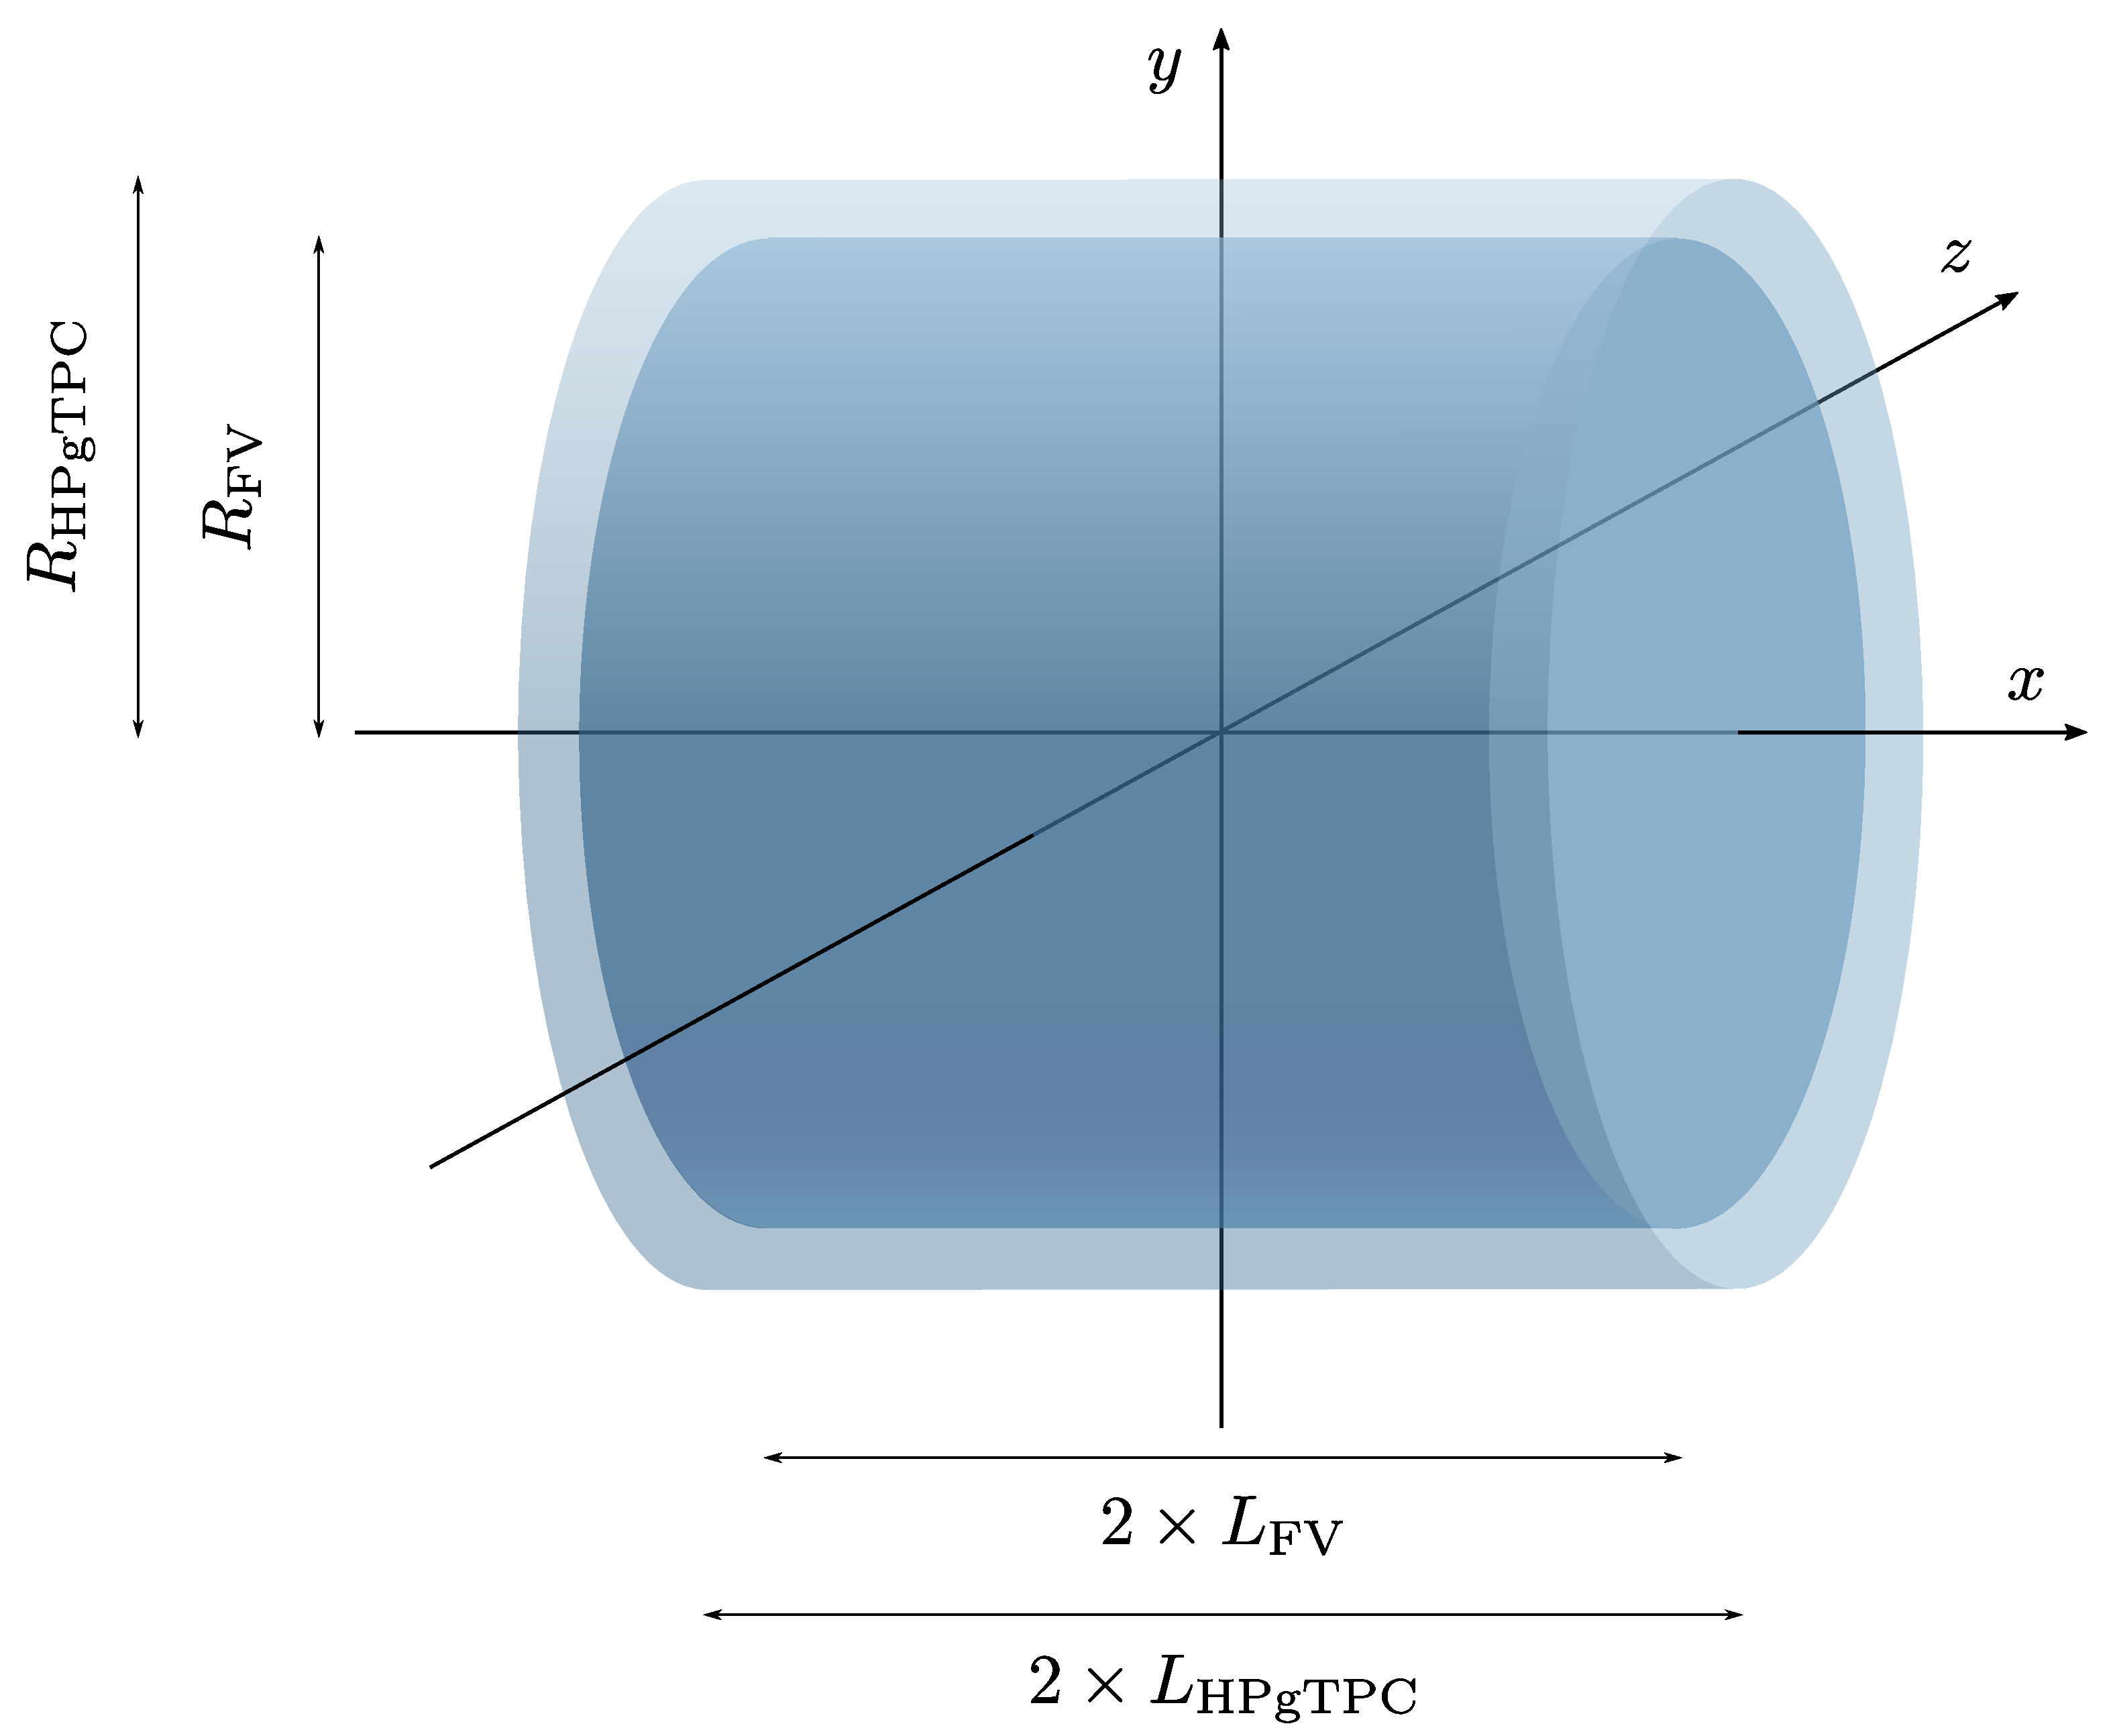
\includegraphics[width=.90\linewidth]{Images/GAr_selection/ndgar_ana_geometry.pdf}
\caption[Schematic diagram of the HPgTPC including the fiducial volume.]{Schematic diagram of the HPgTPC including the fiducial volume (FV). In this case the FV is given by $\Delta L_{\mathrm{FV}} = 30.0 ~ \mathrm{cm}$ and $\Delta R_{\mathrm{FV}} = 30.0 ~ \mathrm{cm}$.}
\label{fig:ndgar_ana_geometry}
\end{figure}

For a particle position to lie within the FV it must satisfy:
\begin{equation}
    \vec{x}_{\mathrm{start}} \in \left\{\vec{x} \in \mathbb{R}^{3} \mid |x_{0}| \leq L_{\mathrm{FV}} ~ \& ~ \sqrt{x_{1}^{2}+x_{2}^{2}} \leq R_{\mathrm{FV}}\right\},
\end{equation}
in the reference frame of the HPgTPC. For convenience, I define:
\begin{equation}
    \begin{split}
        \Delta R_{\mathrm{FV}} &= R_{\mathrm{HPgTPC}} - R_{\mathrm{FV}}, \\
        \Delta L_{\mathrm{FV}} &= L_{\mathrm{HPgTPC}} - L_{\mathrm{FV}},
    \end{split}
\end{equation}
where $R_{\mathrm{HPgTPC}}$ and $L_{\mathrm{HPgTPC}}$ refer to the radius and the half-length of the HPgTPC, respectively.

The key to the CC selection is the identification of a primary muon candidate. Typically, this is the longest track in the event. However, sometimes protons and pions leave tracks longer than that of the muon. This is particularly important in the GAr medium, considerably less dense than the LAr. For this reason, the muon identification in ND-GAr relies mainly on the capabilities of the ECal.

\begin{enumerate}
    \item Event contains reconstructed particles.
    \item Select particles with reconstructed negative charge, $q_{\mathrm{reco}} = -1$.
    \item Select particles passing the muon score cut, $\mu_{\mathrm{score}} \geq \mu_{\mathrm{score}}^{\mathrm{cut}}$.
    \item Keep reconstructed particle with the highest momentum, $\mathrm{max}\left[p_{\mathrm{reco}}\right]$.
    \item Alternatively, keep reconstructed particle with the highest muon score, $\mathrm{max}\left[\mu_{\mathrm{score}}\right]$.
    \item Check that the particle starts within the FV.
\end{enumerate}

\begin{table}[t]
	\caption{Event rates in ND-GAr.}
	\begin{center}
		\begin{small}
			\begin{tabular}{l|lll}
                Cut \# & Selection cut                       & Events & Passing rates          \\[2mm] \hline
                \rule{0pt}{1.1\normalbaselineskip}0      & Total number of events (No cuts)    & 100000 & $100.00\% ~(100.00\%)$ \\[2mm]
                1      & At least one reconstructed particle & 85680  & $85.68 \% ~(85.68 \%)$ \\[2mm]
                2      & Negatively charged particles only   & 62054  & $62.05\% ~(72.43\%)$   \\[2mm]
                3      & $\mu_{\mathrm{score}} >$ threshold  & 45035  & $45.03\% ~(72.57\%)$   \\[2mm]
                4      & $\vec{x}_{\mathrm{start}}$ in FDV   & 31212  & $31.21\% ~(69.31\%)$  
                \end{tabular}
		\end{small}
	\end{center}
	\label{tab:numuCC_selection}
\end{table}

\begin{figure}[t]
	\centering
	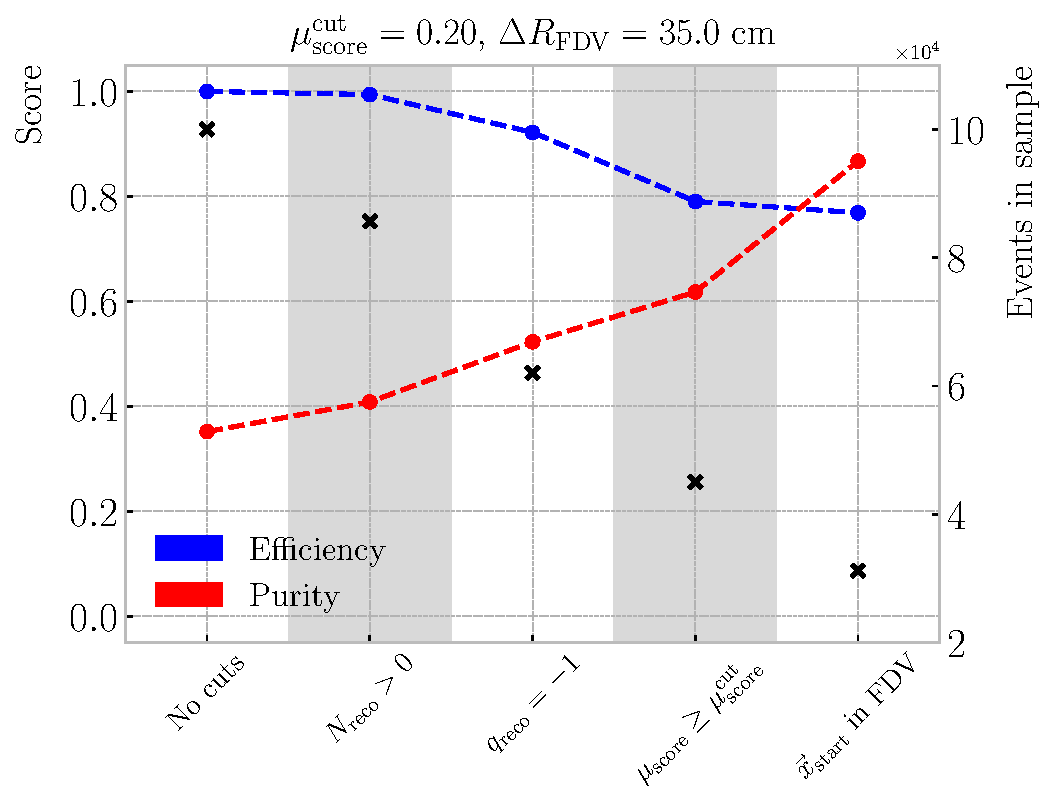
\includegraphics[width=.90\linewidth]{Images/GAr_selection/numu_cc_selection_steps.pdf}
	\caption{}
	\label{fig:numuCC_selection_steps}
\end{figure}

\section{Charged pion identification}

\subsection[\texorpdfstring{$\nu_{\mu}$}{numu} CC \texorpdfstring{$1\pi^{\pm}$}{1pi} selection]{\boldmath\texorpdfstring{$\nu_{\mu}$}{numu} CC \boldmath\texorpdfstring{$1\pi^{\pm}$}{1pi} selection}